\newpage
\section{Diagrams}
\subsection{Class Diagram}
\begin{figure}[h]
	\centerline{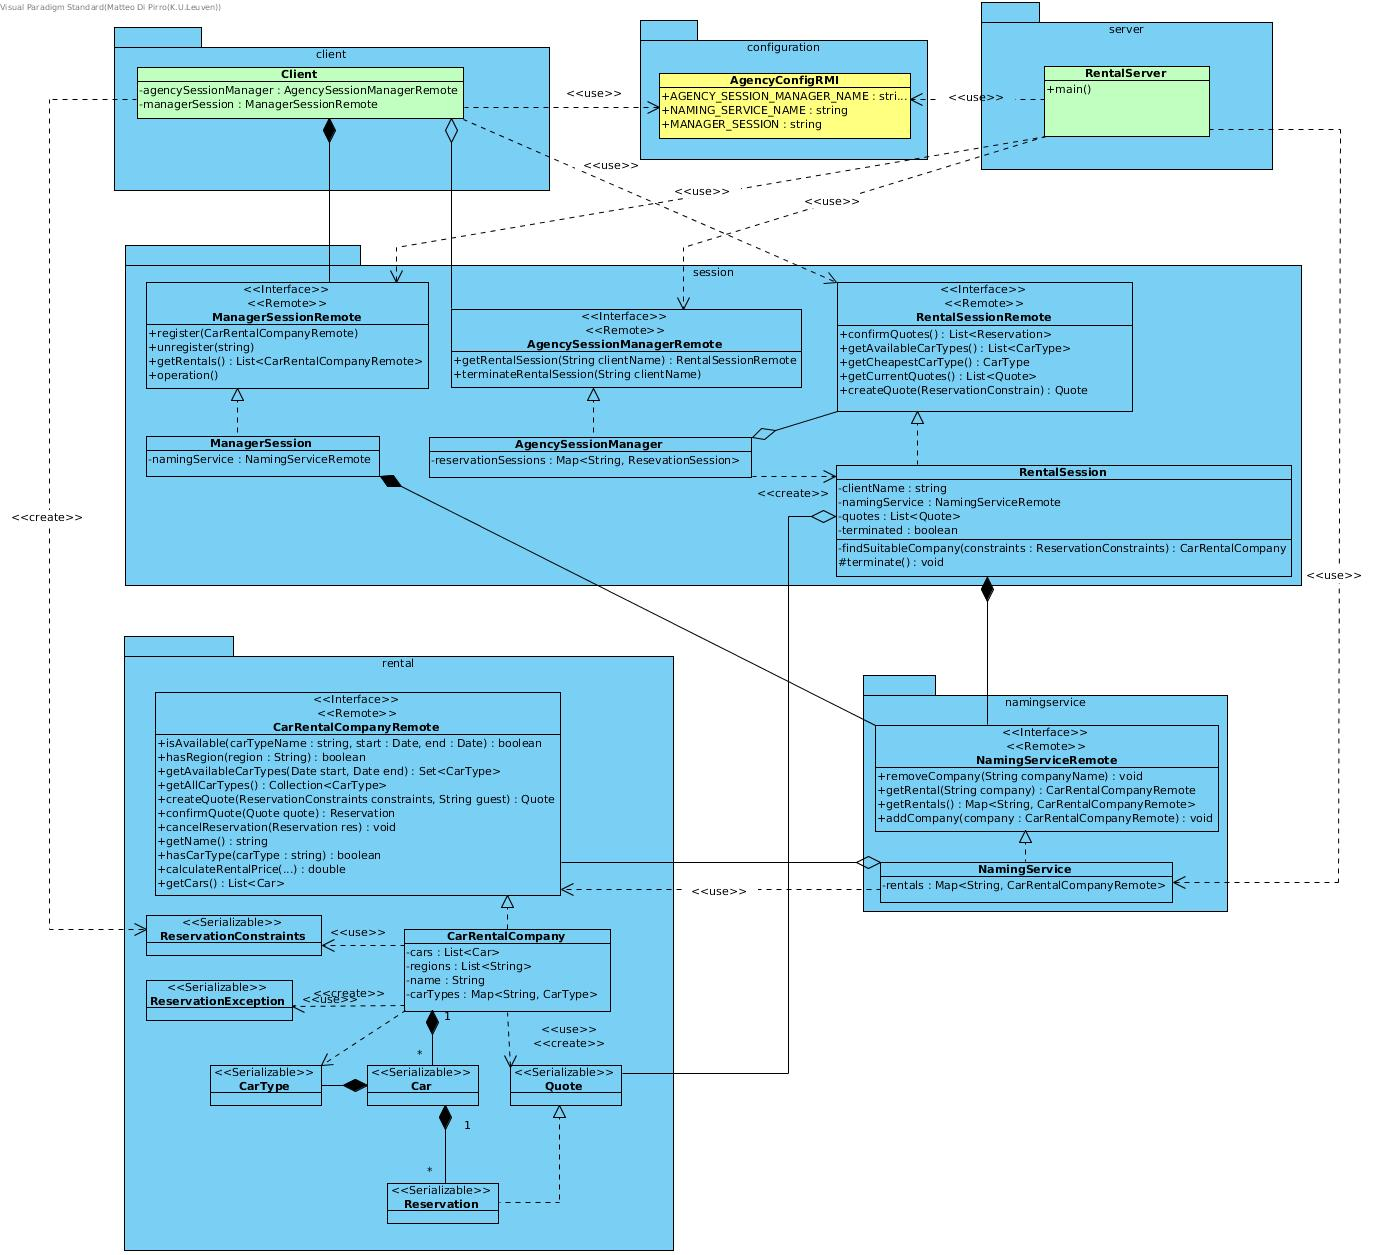
\includegraphics[scale=0.4]{images/classDiagram}}
	\caption{Class Diagram of the car rental application.}
\end{figure}

\newpage
\subsection{Deployment Diagram}
\begin{figure}[h!]
	\centerline{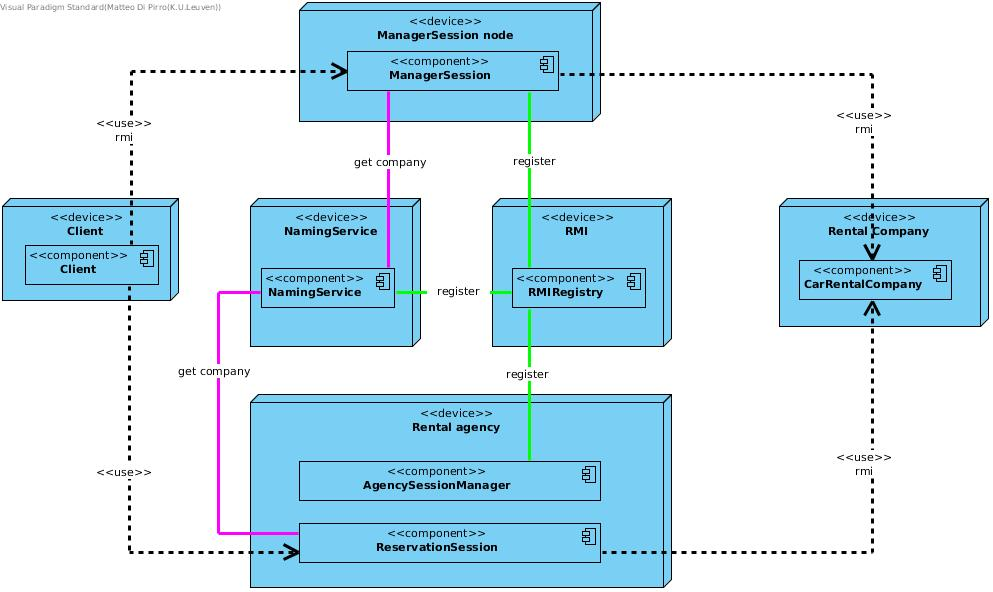
\includegraphics[scale=0.58]{images/deploymentDiagram}}
	\caption{Deployment diagram of the car rental application. Lines representing method invocations are purple colored; lines representing objects bound with the rmi registry are green colored.}
\end{figure}

\newpage
\subsection{Sequence Diagrams}
\subsubsection{Scenario 1 - New rental session}
\begin{figure}[h!]
	\centerline{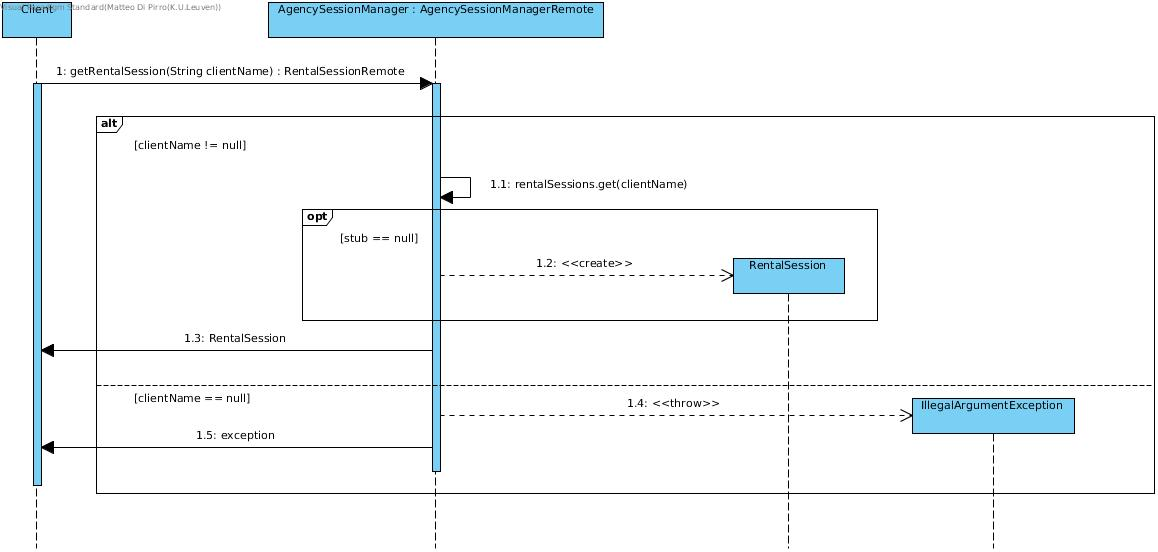
\includegraphics[scale=0.4]{images/newSession}}
	\caption{Sequence diagram for a new rental session scenario.}
\end{figure}

\subsubsection{Scenario 2 - Quotes creation}
\begin{figure}[h!]
	\centerline{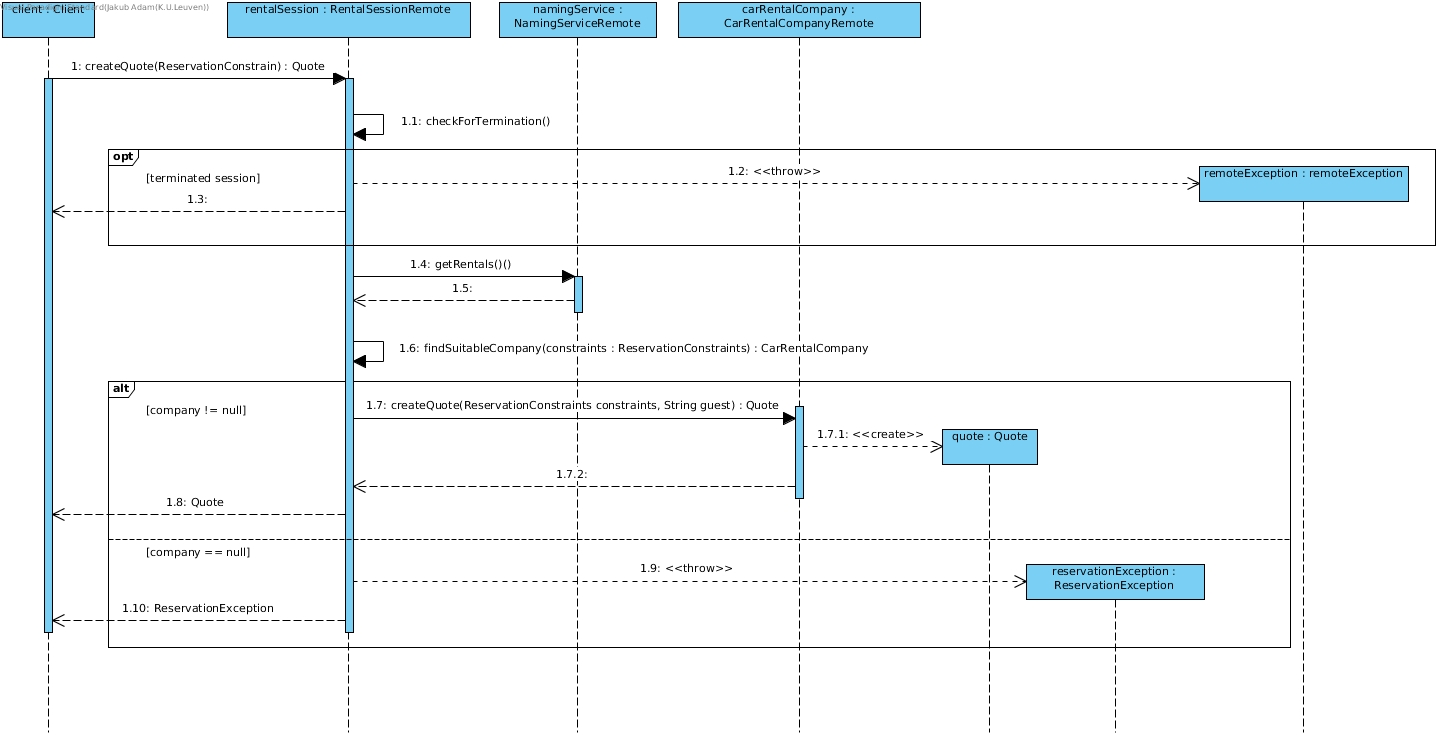
\includegraphics[scale=0.37]{images/quotes}}
	\caption{Sequence diagram for the creation of new quotes at companies A and B.}
\end{figure}

\newpage
\subsubsection{Scenario 3 - Quotes confirmation}
\begin{figure}[h!]
	\centerline{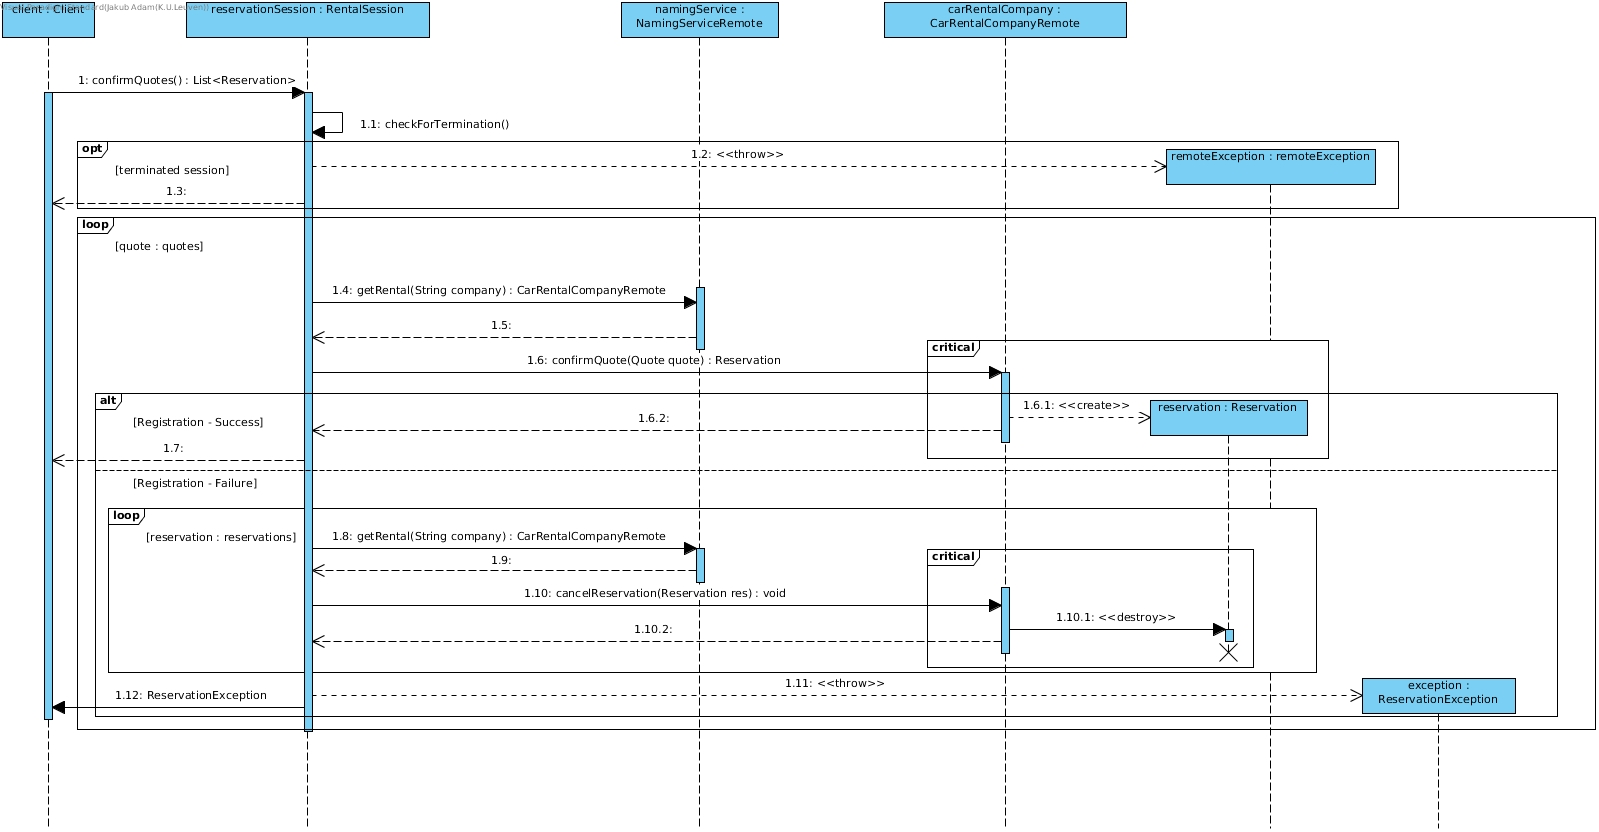
\includegraphics[scale=0.36]{images/confirmation}}
	\caption{Sequence diagram for a quotes confirmation attempt.}
\end{figure}